\documentclass{mcmthesis}

  \makeatletter
  \newcommand{\rmnum}[1]{\romannumeral #1}
  \newcommand{\Rmnum}[1]{\expandafter\@slowromancap\romannumeral #1@}
  \makeatother

\mcmsetup{CTeX = false,   % 使用 CTeX 套装时,设置为 true
        tcn = 0025, problem = A,
        sheet = true, titleinsheet = true, keywordsinsheet = true,
        titlepage = false, abstract = true}
\usepackage{palatino}
\usepackage{lipsum}
\usepackage{amsmath}  
\usepackage{amssymb}
\usepackage{indentfirst} 

\setlength{\parindent}{1.5em}

\title{unsure}
\begin{document}
\begin{abstract}
\lipsum[1]
\begin{keywords}
keyword1; keyword2
\end{keywords}
\end{abstract}
\maketitle
\section{Introduction}
\subsection{Background}

With the rapid development of artificial intelligence, there are more and more applications of images, such as face recognition and automatic recognition. There are two things that cannot be ignored before using images for related tasks.The first is image compression, in order to reduce the redundant information in image data and to store and transmit data in a more efficient format; the second is image restoration, which USES certain techniques to reproduce the missing information in the image.  These two technologies have laid a foundation for the rapid development of relevant image application technologies. In this context, we want to be able to build a process model to implement these two technologies.

\subsection{Restatement of Problem}

We are required to build some mathematical model to process the data of images:
\begin{itemize}
\item A lossy image compression model
\item An inpainting model to recover the image with 20\% missing information.
\item A model to compress a surveillance video in a shopping mall.
\end{itemize}

\subsection{Overview of Our Work}

First, we find a few key points in these questions :
\begin{itemize}
  \item The image compression we need to do is lossy compression.
  \item How to make image compression model suitable for general situation?
  \item What is the relationship between the models we want to build?
  \item Does the missing data proportion have special meaning?
  \item What is the measure of restoration?
  \item All missing pixel values for a given image are non-zero.
  \item How to deal with the static background of video?
\end{itemize}

\section{Assumptions}
\begin{itemize}
  \item We are dealing with bitmaps rather than vectors.
  \item Assume that the missing types of information in question 3 are the same as those in the case diagram.
  \item Assume that the image the image compression algorithm to process is not too extreme for the its size, that is, the image size is not too small or too large.
  \item Assume the image compression algorithm is aimed at the image of RGB color.
  \item Assume that the image compression requires not to lose too much information, not considering the high compression of the signal loss.
\end{itemize}

\section{Notations}

\section{Our Model}
\subsection{Model \Rmnum{1}}
For a digital image using RGB color mode, we first separate the three color channels of red, green and blue.The image data of each channel can be represented by a 2-dimensional matrix. Each element in the 2-dimensional matrix corresponds to one pixel, and its value is the pixel's gray value. After obtaining the three 2-dimensional matrices, We first convert it from RGB to YCbCr. Where Y is the brightness component, Cb is the blue color component, and Cr is the red color component.The human eye is more sensitive to the Y component, so it will be less noticeable to the naked eye when subsampling the chromaticity component to reduce the chromaticity component.YCbCr color space and RGB color space conversion formulas are as follows:
\begin{equation}
\begin{cases}Y=0.299R+0.587G+0.114B\\Cb=0.564(B-Y)\\Cr=0.713(R-Y)\end{cases}
\end{equation}
\begin{equation}
\begin{cases}R=Y+1.402Cr\\G=Y-0.344Cb-0.714Cr\\B=Y+1.772Cb\end{cases}
\end{equation}
We decide use YCbCr 4:2:0 format,which is by far the most common color representation used in compressedimages and video.[1] 

\subsection{Other Assumptions}
\lipsum[6]
\begin{itemize}
\item
\item
\item
\item
\end{itemize}

\lipsum[7]

\section{Analysis of the Problem}
\begin{figure}[h]
\small
\centering
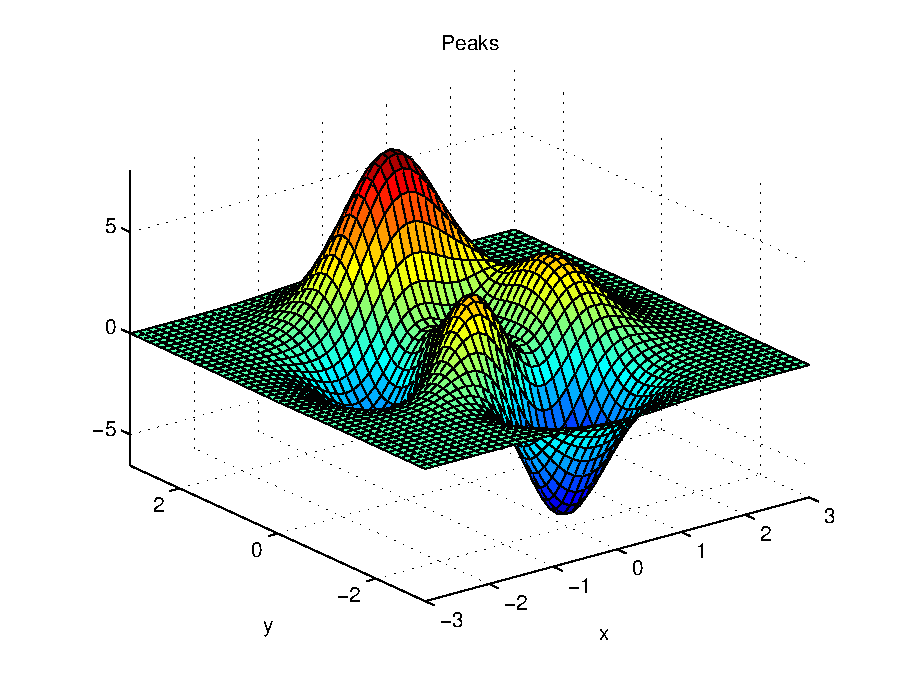
\includegraphics[width=12cm]{mcmthesis-aaa.eps}
\caption{aa} \label{fig:aa}
\end{figure}

\lipsum[8] \eqref{aa}
\begin{equation}
a^2 \label{aa}
\end{equation}

\[
  \begin{pmatrix}{*{20}c}
  {a_{11} } & {a_{12} } & {a_{13} }  \\
  {a_{21} } & {a_{22} } & {a_{23} }  \\
  {a_{31} } & {a_{32} } & {a_{33} }  \\
  \end{pmatrix}
  = \frac{{Opposite}}{{Hypotenuse}}\cos ^{ - 1} \theta \arcsin \theta
\]
\lipsum[9]

\[
  p_{j}=\begin{cases} 0,&\text{if $j$ is odd}\\
  r!\,(-1)^{j/2},&\text{if $j$ is even}
  \end{cases}
\]

\lipsum[10]

\[
  \arcsin \theta  =
  \mathop{{\int\!\!\!\!\!\int\!\!\!\!\!\int}\mkern-31.2mu
  \bigodot}\limits_\varphi
  {\mathop {\lim }\limits_{x \to \infty } \frac{{n!}}{{r!\left( {n - r}
  \right)!}}} \eqno (1)
\]

\section{Calculating and Simplifying the Model  }
\lipsum[11]

\section{The Model Results}
\lipsum[6]

\section{Validating the Model}
\lipsum[9]

\section{Conclusions}
\lipsum[6]

\section{A Summary}
\lipsum[6]

\section{Evaluate of the Mode}

\section{Strengths and weaknesses}
\lipsum[12]

\subsection{Strengths}
\begin{itemize}
\item \textbf{Applies widely}\\
This  system can be used for many types of airplanes, and it also
solves the interference during  the procedure of the boarding
airplane,as described above we can get to the  optimization
boarding time.We also know that all the service is automate.
\item \textbf{Improve the quality of the airport service}\\
Balancing the cost of the cost and the benefit, it will bring in
more convenient  for airport and passengers.It also saves many
human resources for the airline. \item \textbf{}
\end{itemize}

\begin{thebibliography}{99}
\bibitem{1} D.~E. KNUTH   The \TeX{}book  the American
Mathematical Society and Addison-Wesley
Publishing Company , 1984-1986.
\bibitem{2}Lamport, Leslie,  \LaTeX{}: `` A Document Preparation System '',
Addison-Wesley Publishing Company, 1986.
\bibitem{3}\url{http://www.latexstudio.net/}
\bibitem{4}\url{http://www.chinatex.org/}
\end{thebibliography}

\begin{appendices}

\section{First appendix}

\lipsum[13]

Here are simulation programmes we used in our model as follow.\\

\textbf{\textcolor[rgb]{0.98,0.00,0.00}{Input matlab source:}}
\lstinputlisting[language=Matlab]{./code/mcmthesis-matlab1.m}

\section{Second appendix}

some more text \textcolor[rgb]{0.98,0.00,0.00}{\textbf{Input C++ source:}}
\lstinputlisting[language=C++]{./code/mcmthesis-sudoku.cpp}

\end{appendices}
\end{document}

%% 
%% This work consists of these files mcmthesis.dtx,
%%                                   figures/ and
%%                                   code/,
%% and the derived files             mcmthesis.cls,
%%                                   mcmthesis-demo.tex,
%%                                   README,
%%                                   LICENSE,
%%                                   mcmthesis.pdf and
%%                                   mcmthesis-demo.pdf.
%%
%% End of file `mcmthesis-demo.tex'.
